\chapter{Detectability in IM Surveys}
\label{chapter:snrska}

We investigate the detectability of leading-order relativistic effects in the bispectrum of future 21cm intensity  mapping surveys. The relativistic signal arises from Doppler and other line-of-sight effects in redshift space. In the power spectrum of a single tracer, these effects are suppressed by a factor $\cH^2/k^2$. By contrast, in the bispectrum the relativistic signal couples to short-scale modes, leading to
an imaginary contribution that scales as $\cH/k$, thus increasing the possibility of detection.
Previous work has shown that this relativistic signal is detectable in a Stage IV H$\alpha$ galaxy survey. 
{We show that the signal is also detectable by next-generation  21cm intensity maps, but typically with a lower signal-to-noise, due to foreground and telescope beam effects.}
%
%
%---------------------------
%
%
\section{Introduction}

{Next-generation galaxy surveys will allow for precision measurements of the  bispectrum, bringing new information to improve constraints on cosmological parameters and to break some of their degeneracies (see e.g. \cite{Scoccimarro:2015bla,Tellarini:2016sgp, Gil-Marin:2016wya,  Slepian:2016kfz,Gagrani:2016rfy, Sugiyama:2018yzo,Desjacques:2018pfv,Child:2018klv, Yankelevich:2018uaz, Schmit:2018rtf,DiDio:2018unb,Gualdi:2019ybt,Sarkar:2019ojl,Chudaykin:2019ock,Oddo:2019run, Sugiyama:2019ike,Philcox:2019hdi,Durrer:2020orn,Montanari:2020uez}). 

These surveys will typically probe very large volumes in the Universe, including ultra-large scales ($k\lesssim k_{\mathrm{eq}} \sim 0.01\;\mathrm{Mpc}^{-1}$), which facilitates the detection of, or precision constraints on, primordial non-Gaussianity \cite{Tellarini:2015faa,Watkinson:2017zbs,Majumdar:2017tdm,Karagiannis:2018jdt,Karagiannis:2019jjx,Bharadwaj:2020wkc}
and relativistic effects
\cite{Kehagias:2015tda,Umeh:2016nuh, DiDio:2016gpd, Jolicoeur:2017nyt,Bertacca:2017dzm,Jolicoeur:2017eyi,Koyama:2018ttg,Clarkson:2018dwn,Maartens:2019yhx,Jeong:2019igb}.
 
Redshift-space distortions (RSD) are the dominant observational effect on the number counts or brightness temperature at first and second order in perturbations. There are local relativistic corrections to standard RSD, arising from Doppler and other line-of-sight gradient terms, together with their couplings.  In Fourier space, the leading-order corrections  scale as i\,$(\cH/k)$. In the tree-level power spectrum of a single tracer, the only nonzero contribution from these Doppler-type effects is from their square, since the power spectrum is necessarily real. As a result, the Doppler-type effects are further suppressed in the auto-power spectrum, scaling as  $(\cH/k)^2$. 

The tree-level bispectrum of a single tracer is not forced to be real and it couples Doppler-type effects with the standard (`Newtonian') density + RSD term. Consequently, the leading-order relativistic contribution to the bispectrum scales as i\,$(\cH/k)$. 
This means that the leading-order relativistic signal is more detectable in the bispectrum than the power spectrum, for a single tracer.
In Fourier space, the dominant relativistic effect is a purely imaginary part of the bispectrum, as shown by \cite{Clarkson:2018dwn,Maartens:2019yhx}. Our previous work \cite{Maartens:2019yhx} showed that it is detectable by a Stage IV spectroscopic galaxy survey.

 In this work, we investigate the detectability of the relativistic signal in the bispectrum of various planned 21cm intensity mapping surveys at post-reionisation redshifts. 
The 21cm emission line of neutral hydrogen (HI) is measured without detecting the individual galaxies that contain HI. This results in brightness temperature maps that trace the large-scale structure with exquisite redshift precision. In Section 2 we discuss the leading order relativistic form of the temperature contrast up to second order, and its contribution to the bispectrum. Section 3 describes the signal, modelled using the tree-level bispectrum with the addition of a phenomenological model to account for RSD `fingers-of-god' nonlinearity.
Foreground contamination overwhelms the signal, and cleaning techniques must be applied which lead to a loss of signal in regions of Fourier space, which we take into account. We also discuss the effects of telescope beams and the instrumental noise. Our forecast signal to noise for future surveys is presented in Section 4, and we conclude in Section 5.}
%
%
%---------------------------------------------
%
%
\section{Relativistic effects in the 21cm intensity bispectrum}
%
{The HI brightness temperature  measured at redshift $z$ in direction $\n$  is related to the observed number of 21cm emitters per redshift per solid angle, $N_{\hi}$, as follows (see \cite{Hall:2012wd,Alonso:2015uua} for details):
\begin{equation}
T_{\hi}(z,\n)= {\mathrm{const.}}\, \frac{ N_{\hi}(z,\n)}{d_{\mathrm{A}}(z,\n)^2}\,,
\label{tobs}
\end{equation}
where $d_{\mathrm{A}}$ is the angular diameter distance.  

{The background HI brightness temperature  follows from \eqref{tobs} as \cite{Villaescusa-Navarro:2018vsg}
\begin{equation} \label{bart}
\bar{T}_{\mathrm{HI}}(z)= 189h\,\frac{(1+z)H_0}{\HH(z)}\Omega_{\hi}(z)~~{\mathrm{mK}}.
\end{equation}
Here $h=H_0/(100\,$km/s), $\HH=(\ln a)'$ is the conformal Hubble rate, and $\Omega_{\hi}(z)$ is the comoving HI density in units of the critical density today, which is currently poorly constrained by observations and is modelled by simulations. We use the fit 
%in \cite{Bacon:2018dui}, $\Omega_{\hi}=(4.8+3.9\,z-0.65\,z^2)\times 10^{-4}$, and then
in  \cite{Santos:2017qgq}:
\begin{equation}
\bar{T}_{\mathrm{HI}}(z) = 0.0 56 +0.23\,z -0.024\, z^{2} ~~ \mathrm{mK}. \label{e1.24}
\end{equation}}

% %
The temperature fractional perturbation is
\begin{equation}
\Delta_{\hi}(z,\bm{n}) = \frac{T_{\hi}(z,\bm{n}) - \bar {T}_{\hi} (z)}{\bar {T}_{\hi} (z)}\,.\label{e1.1_02}
\end{equation}
Using \eqref{tobs}, this leads to the following perturbative expansion (our convention is $X+X^{\tw}/2$).
\begin{itemize}
\item
{\bfseries At first order} \cite{Hall:2012wd}:
\begin{equation} \label{dt1}
\Delta \equiv \Delta^{(1)}_{\hi} = \Delta_{\mathrm{N}} + \Delta_{\mathrm{D}}\,,\quad  \Delta_{\mathrm{N}} = b_1\delta_{\mathrm{m}} - \frac{1}{\HH}\p_r(\v\cdot\n )\,,\quad \Delta_{\mathrm{D}}=A\,(\v\cdot\n ) \,.
\end{equation}
Here   $r$ is the radial comoving distance and $\v=\bm{\nabla}V$ is the peculiar velocity.
$ \Delta_{\mathrm{N}} $ is the standard density + RSD term, which scales as $\delta_{\mathrm{m}}$. $\Delta_{\mathrm{D}}$ is the dominant relativistic correction, scaling as i\,$(\cH/k)\delta_{\mathrm{m}}$ in Fourier space. This Doppler term has coefficient
\begin{equation}
A = b_{\mathrm{e}} - 2- \frac{\cH'}{\cH^{2}}= - \frac{\ud \ln \big[(1+z) \bar{T}_{\hi} \big]}{\ud \ln (1+z)} \,,
 \label{eq:dopcoeff}
\end{equation}
where  the evolution bias is \cite{Fonseca:2015laa}
\begin{equation}
 b_{\mathrm{e}} = - \frac{\ud \ln \big[(1+z)^{-1}\HH\, \bar{T}_{\hi} \big] }{\ud \ln (1+z)}\,.
\end{equation}
We omit sub-leading relativistic corrections that scale as $(\HH/k)^2\delta_{\mathrm{m}}$. 


\item
{\bfseries At second order}
\cite{Maartens:2019yhx} (see also \cite{Umeh:2015gza,DiDio:2015bua,Umeh:2016thy,Clarkson:2018dwn,DiDio:2018zmk}):
\begin{align}
\Delta^{\tw} &\equiv  \Delta^{(2)}_{\hi} = \Delta^{\tw}_{\mathrm{N}} + \Delta^{\tw}_{\mathrm{D}} \,,\\
\Delta^{\tw}_{\mathrm{N}}&= b_1\delta_{\mathrm{m}}^{\tw}+b_2 \big(\delta_{\mathrm{m}}\big)^2+ b_{s^2}s^2 + {\mathrm{RSD}}^{\tw}\,,
\label{d2n} \\
\Delta^{\tw}_{\mathrm{D}} &= A\, (\bm{v}^{(2)}\!\!\cdot\bm{n})+2\Big[ b_{1}\big(A+f) + \frac{b_1'}{\cH}\Big]\,(\bm{v}\cdot\bm{n})\,\delta_{\mathrm{m}} +\frac{1}{\cH}\big( 8-4A-3\Omega_{\mathrm{m}}   \big)(\bm{v}\cdot\bm{n})\,\partial_r(\bm{v}\cdot\bm{n})
\nonumber\\ \label{e1.2}
& +\frac{2}{\cH^2}\big[(\bm{v}\cdot\bm{n}) \,\partial_r^2\Phi-\Phi\, \partial_r^2 (\bm{v}\cdot\bm{n}) \big]
 -\frac{2}{\cH}\,\partial_r (\bm{v}\cdot\bm{v})+2 \frac{{b_{1}}}{\cH}\,\Phi\, \partial_r\delta_{\mathrm{m}} \,.
\end{align}
In \eqref{d2n}, $b_{s^2}s^2$ is the tidal bias contribution and RSD$^{\tw}$ is the standard second-order RSD contribution (see \cite{Maartens:2019yhx} for details). The bias parameters are computed via a halo model (see  Appendix REFERENCE APPENDIX 1) and are shown in Figure \ref{fig:hibiasT}, together with the evolution bias.
In \eqref{e1.2}, we see the Doppler terms and the line-of-sight gradients that make up the dominant relativistic contribution.
$\Phi$ is the gravitational potential and $\Omega_{\mathrm{m}} =\Omega_{{\mathrm{m}}0}(1+z)H_0^2/\cH^2$. We  neglect sub-dominant relativistic effects in $\Delta^{\tw}$ that scale as  $(\cH/k)^2(\delta_{\mathrm{m}})^2$. 

%
%\vspace*{-0.5cm}
\begin{figure}[ht]
\centering
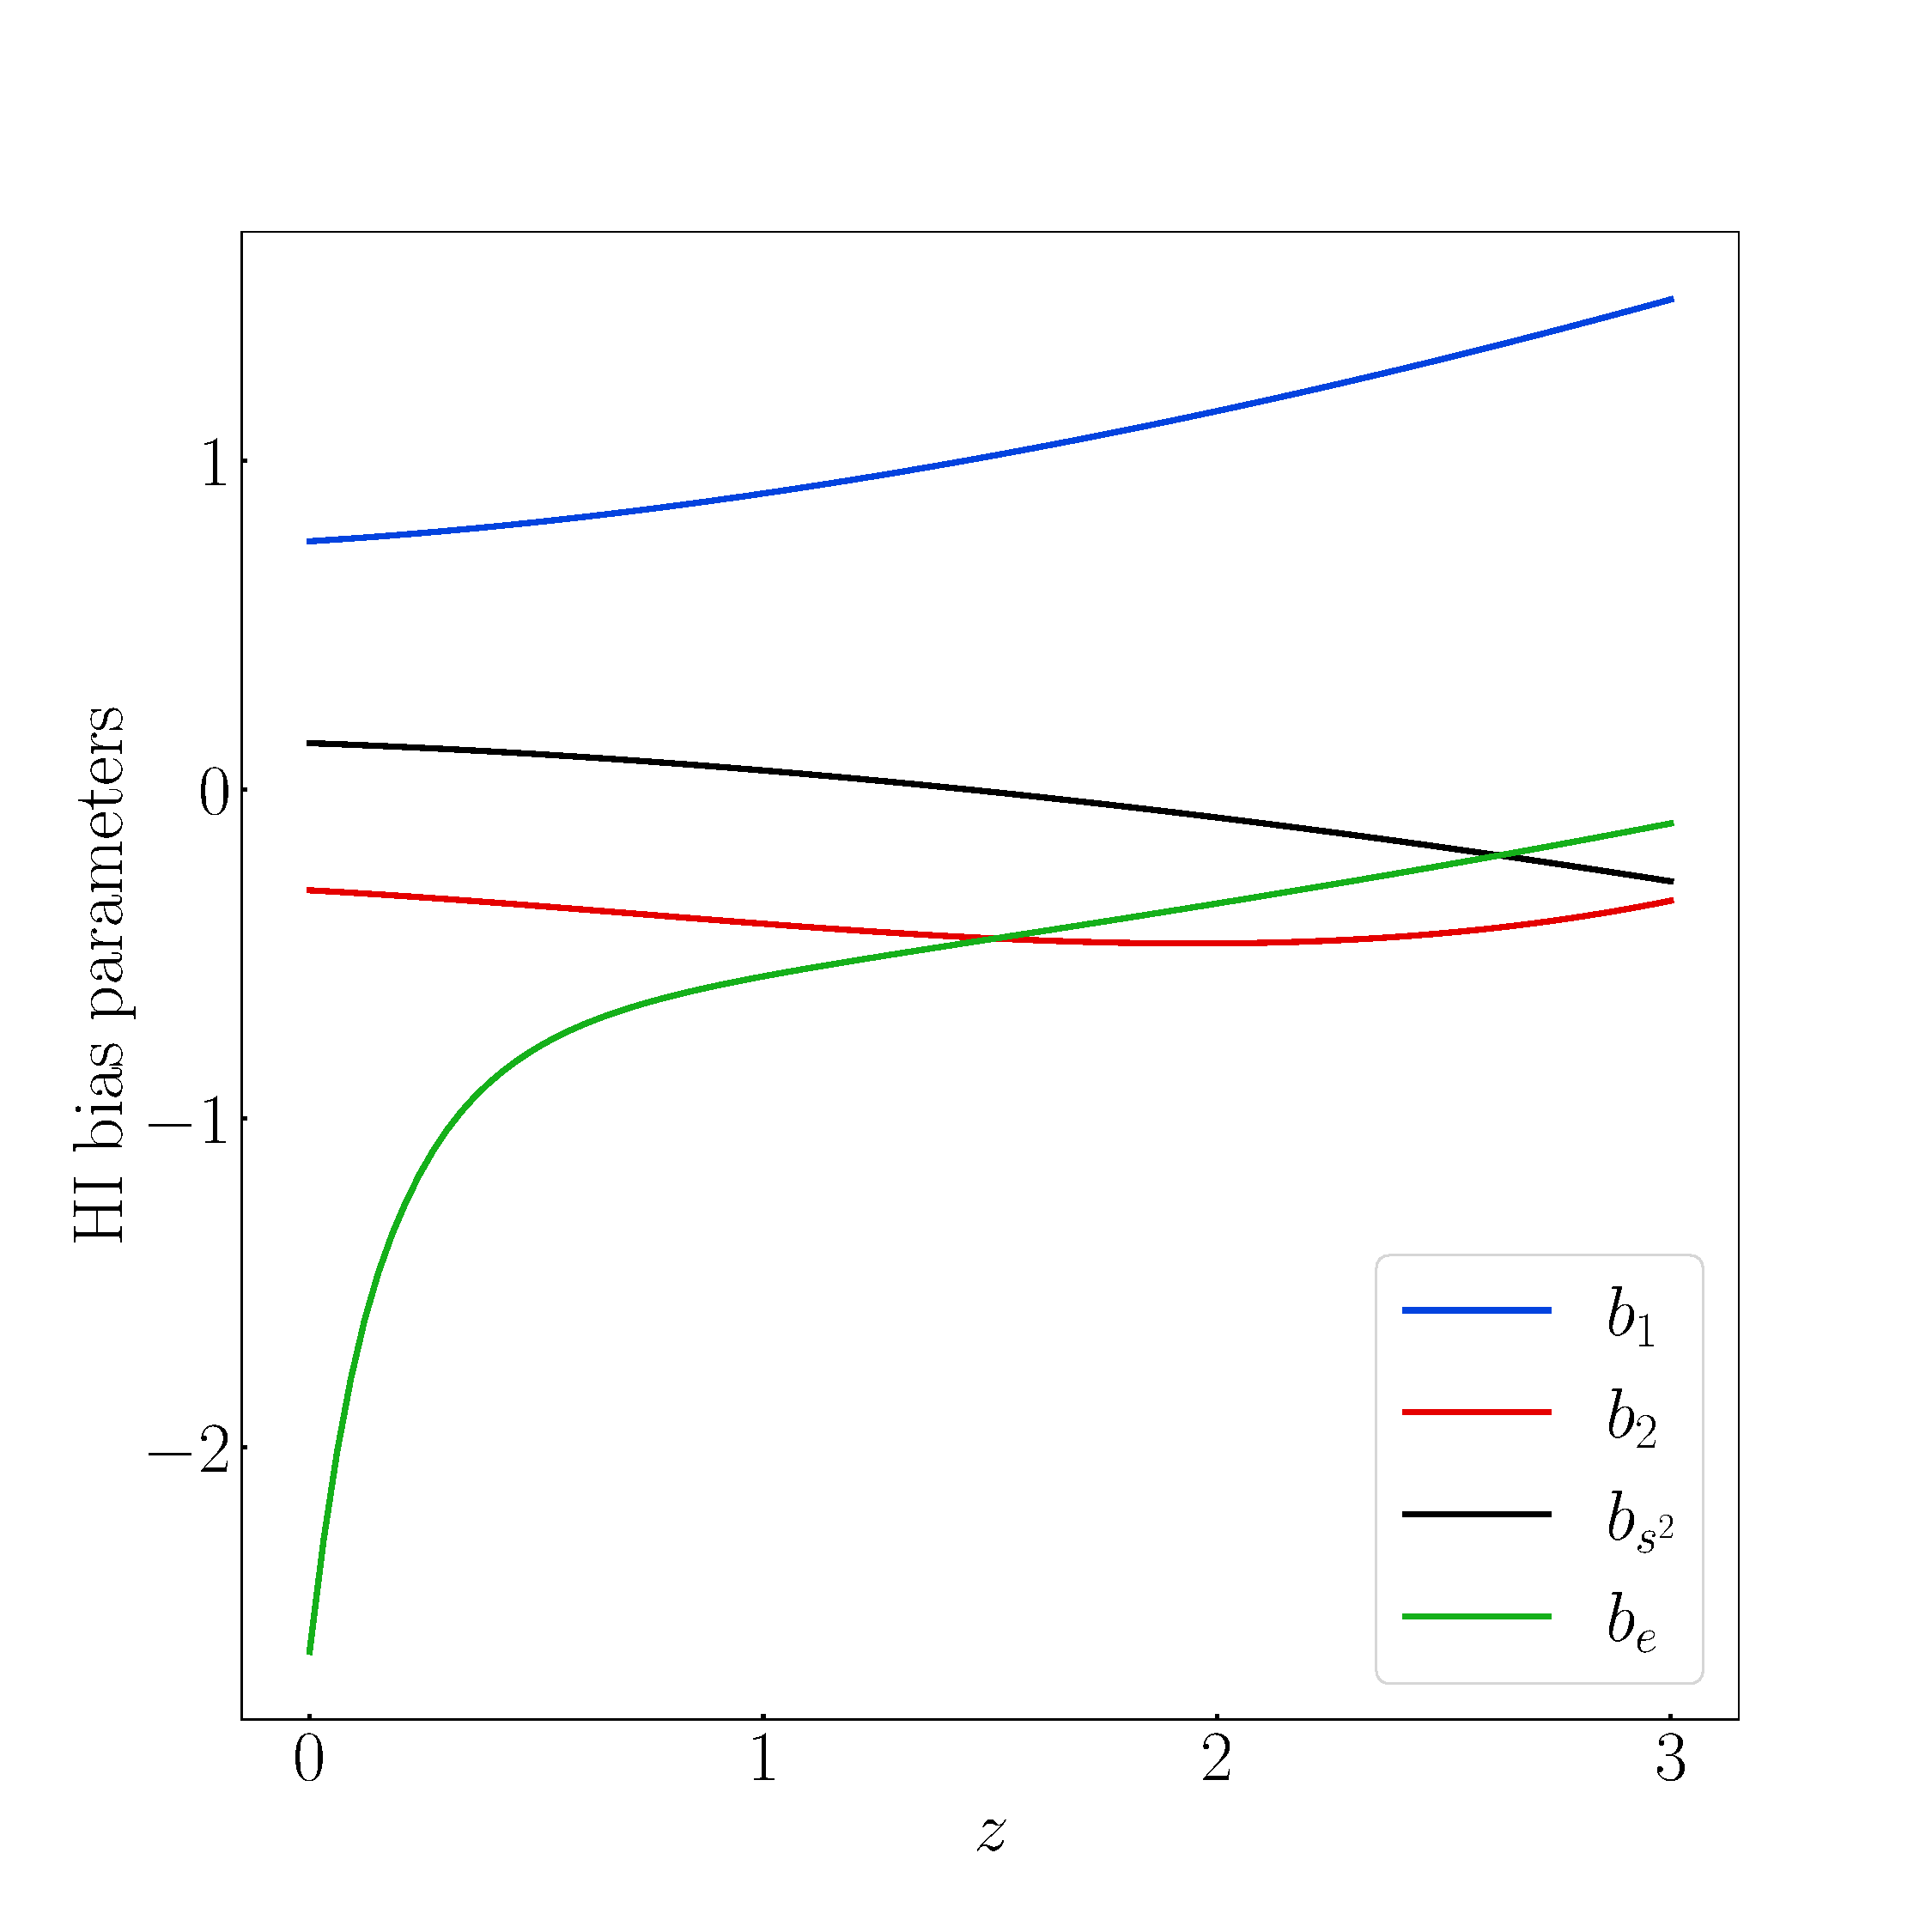
\includegraphics[width=.49\textwidth]{fig/HIBias}
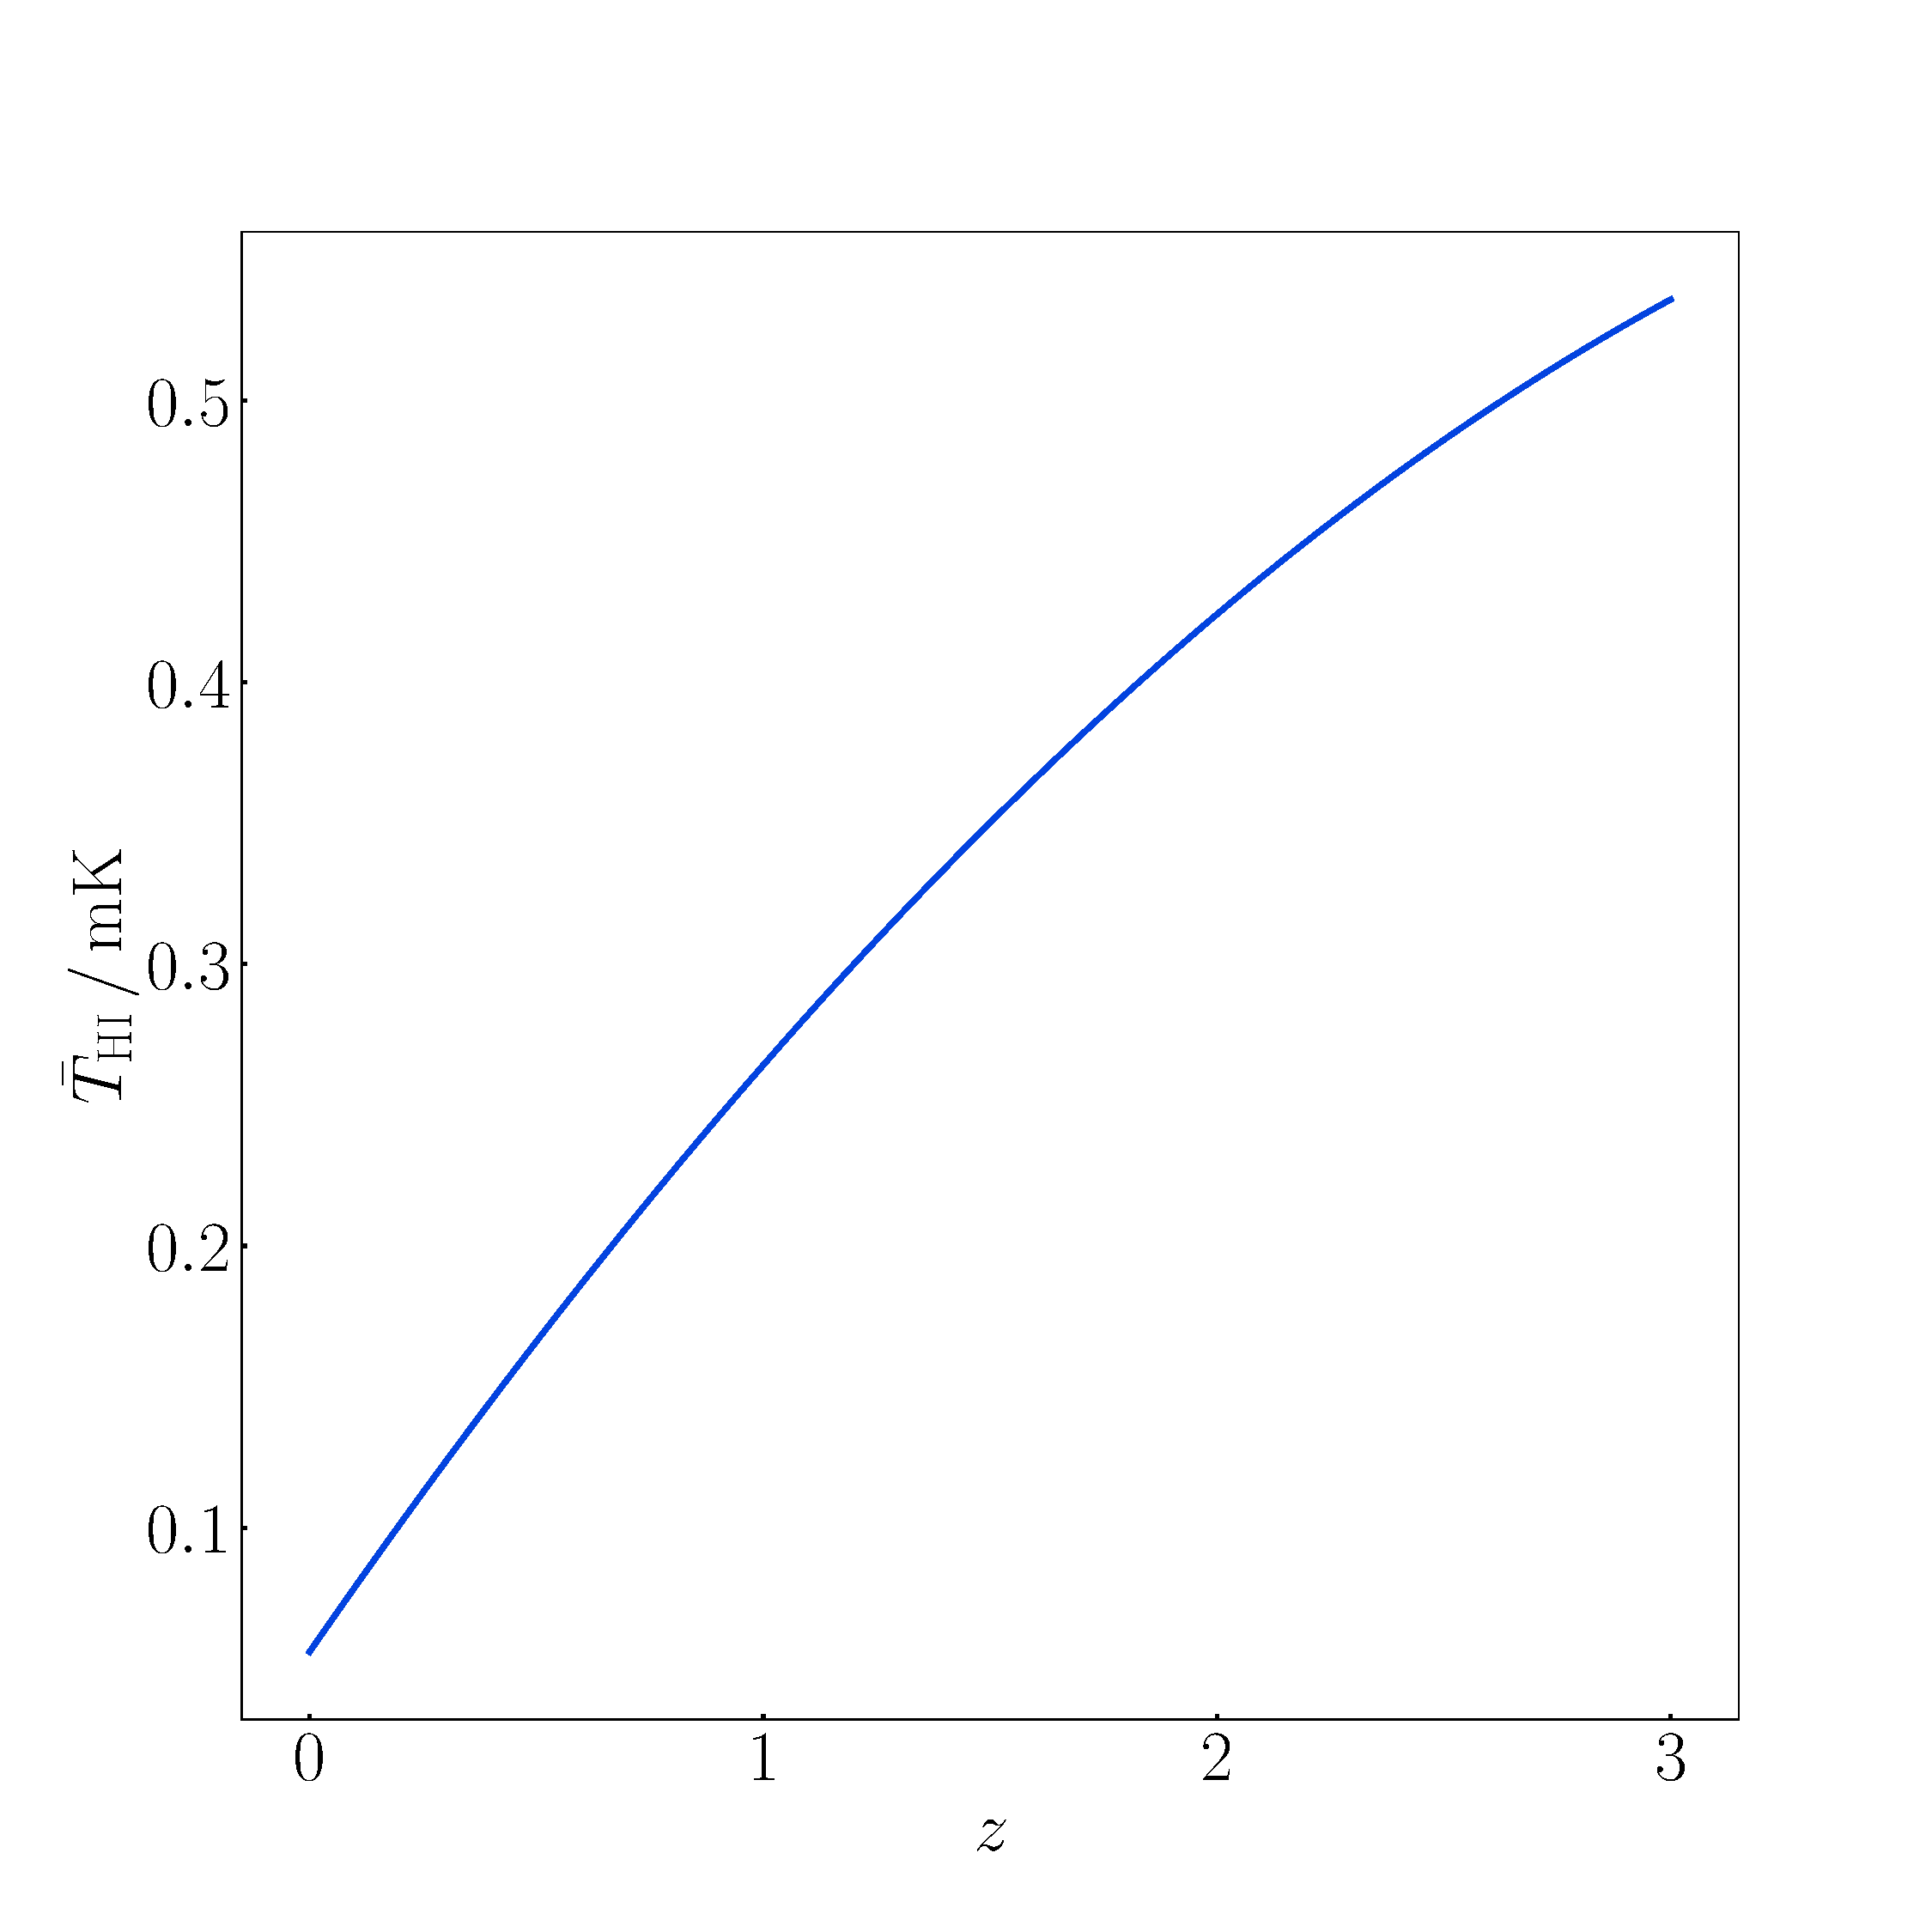
\includegraphics[width=.49\textwidth]{fig/THI.pdf}
%\vspace*{-0.5cm}
\caption{HI clustering and evolution bias parameters (left) and background temperature (right).}\label{fig:hibiasT}
\end{figure}

\item {\bfseries Lensing contribution:}\\
At first order, there is no lensing contribution to $\Delta$ \cite{Hall:2012wd}. The general case of galaxy number density contrast contains a lensing  contribution $2({\cal Q}-1)\kappa$ to $\Delta_g$, where $\kappa$ is the convergence \cite{Challinor:2011bk}.  For HI emitters in intensity mapping, the magnification bias satisfies
\begin{equation}
{\cal Q} \equiv - \frac{\p \ln \bar{N}_{\hi}}{\p \ln L}\bigg|_{\mathrm{c}} = 1\,, \label{magb}
\end{equation}
where c indicates evaluation at the luminosity cut. 

At second order,  \eqref{tobs} shows that there is also no contribution to $\Delta^{\tw}$ from lensing convergence \cite{DiDio:2015bua,Jalivand:2018vfz}. We can recover this result from the full general expression for second-order number density contrast  \cite{Bertacca:2014dra, Bertacca:2014wga, Yoo:2014sfa, DiDio:2014lka, Bertacca:2014hwa}, by imposing \eqref{magb} together with the conditions \cite{DiDio:2015bua}
\begin{equation} \label{magb2}
\frac{\p^2 \ln \bar{N}_{\hi}}{\p (\ln L)^2}\bigg|_{\mathrm{c}} = 0\,, \quad  \frac{\p b_1}{\p \ln L}\bigg|_{\mathrm{c}}=0\,.
\end{equation}

There remains however a lensing deflection contribution $\nabla_{\perp a}\Delta\,\nabla_\perp^a\phi$ to  $\Delta^{\tw}$,  where $\nabla_{\perp a}$ is a screen-space gradient and $\phi$ is the lensing potential \cite{Umeh:2015gza,DiDio:2015bua,Jalivand:2018vfz}. In the bispectrum the contribution of this term is negligible for equal-redshift correlations \cite{DiDio:2015bua,Durrer:2020orn}. Since we only consider the bispectrum at equal redshifts, we neglect this term. 
\end{itemize}}
% \vspace{0.2cm}

In Fourier space, the  HI bispectrum  at  tree level  is defined by
\begin{equation}
\big\langle \Delta(z,\bm{k}_{1})\Delta(z,\bm{k}_{2})\Delta^{(2)}(z,\bm{k}_{3}) \big\rangle + \text{2 cp}=2 (2\pi)^3 B_{\hi}(z, \bm{k}_{1}, \bm{k}_{2}, \bm{k}_{3}) \delta^{\mathrm{Dirac}}\big(\bm{k}_{1}+ \bm{k}_{2}+ \bm{k}_{3} \big)\,, \label{e1.3}
\end{equation}
where cp denotes cyclic permutation. It follows that
%and the factor 2 on the right is due to the convention that the total HI brightness contrast is $\Delta^{(1)}_{\rm HI}+ \Delta^{(2)}_{\rm HI}/2$. 
\begin{equation}
B_{\hi}(z, \bm{k}_{1}, \bm{k}_{2}, \bm{k}_{3}) = \mathcal{K}^{(1)}(z, \bm{k}_{1})\mathcal{K}^{(1)}(z, \bm{k}_{2})\mathcal{K}^{(2)}(z, \bm{k}_{1}, \bm{k}_{2}, \bm{k}_{3})P_{\mathrm{m}} (z, k_{1})P_{\mathrm{m}} (z, k_{2}) + \text{2 cp}\;, \label{e1.5}
\end{equation} 
where $P_{\mathrm{m}} $ is the linear matter power spectrum (computed using CLASS \cite{Blas:2011rf}).  From now on, we often drop the $z$ dependence for brevity.  
%
The  bispectrum kernels are as follows.
\begin{itemize}
\item
{\bfseries Standard (Newtonian) kernels:}
\begin{align}
\mathcal{K}^{(1)}_{\mathrm{N}}(\bm{k}_{a}) &= b_{1}+f\mu_{a}^{2}\,,  \label{e1.7} \\ 
\mathcal{K}^{(2)}_{\mathrm{N}}(\bm{k}_{1}, \bm{k}_{2},{\bm{k}_3}) &= b_{1}F_{2}(\bm{k}_{1}, \bm{k}_{2}) + b_{2} + f\mu_{3}^{2}G_{2}(\bm{k}_{1}, \bm{k}_{2}) +{fZ_2}(\bm{k}_{1}, \bm{k}_{2})
+ b_{s^{2}}S_{2}(\bm{k}_{1}, \bm{k}_{2})\,, \label{e1.8}
\end{align}
where $f$ is the linear matter growth rate, $\mu_a=\hat{\k}_a\cdot\n$ and the standard $F_2,G_2,Z_2,S_2$ kernels are given in \cite{Maartens:2019yhx}.

\item
{\bfseries Leading-order relativistic kernels:} 
\begin{align}
\mathcal{K}^{(1)}_{\mathrm{D}}(\bm{k}_{a}) &= \mathrm{i}\,\cH f A\,\frac{\mu_{a}}{k_{a}}\,, \label{e1.9} \\
\mathcal{K}^{(2)}_{\mathrm{D}}(\bm{k}_{1},\bm{k}_{2},\bm{k}_{3}) &= \i\,\cH f \bigg\{
A\,\frac{\mu_{3}}{k_{3}}G_{2}(\bm{k}_{1},\bm{k}_{2})
+{\Big[b_1\big(A+f\big)+ \frac{b_1'}{\cH} \Big]}\Big(\frac{\mu_{1}}{k_{1}} + \frac{\mu_{2}}{k_{2}}\Big)
\nonumber \\
&  -\frac{3}{2}\Omega_{\mathrm{m}} \Big(\mu_{1}^{3}\frac{k_{1}}{k_{2}^{2}} + \mu_{2}^{3}\frac{k_{2}}{k_{1}^{2}}\Big)
+{\Big[\frac{3}{2}\Omega_{\mathrm{m}} \big(1+f \big)+2f\big(A-2\big) \Big]}\mu_{1}\mu_{2}\Big(\frac{\mu_{1}}{k_{2}}+\frac{\mu_{2}}{k_{1}}\Big)
\nonumber \\
& +2f\,  {\hat{\bm{k}}_{1} \cdot \hat{\bm{k}}_2}\Big(\frac{\mu_{1}}{k_{1}} + \frac{\mu_{2}}{k_{2}}\Big) 
-\frac{3\Omega_{\mathrm{m}} b_1}{2f}\Big(\mu_{1}\frac{k_{1}}{k_{2}^{2}} + \mu_{2}\frac{k_{2}}{k_{1}^{2}}\Big)\!  \bigg\}\,,\label{e1.10}
\end{align}
where $A$ is given by \eqref{eq:dopcoeff}. These follow from \eqref{dt1} and \eqref{e1.2}, and {agree with \cite{Maartens:2019yhx} when we impose \eqref{eq:dopcoeff}, \eqref{magb} and \eqref{magb2}}.
\item
{\bfseries Complex bispectrum:}\\
From \eqref{e1.7}--\eqref{e1.10} we see that
$B_{\hi}$ is complex: {the imaginary part is given purely by local relativistic corrections, while at leading order, i.e. neglecting relativistic terms of $O(\cH^2/k^2)$, the real part is given purely by the standard Newtonian bispectrum:}
\begin{align}
\mathrm{Re}\big(B_{\hi}\big) &= B_{\mathrm{N}} = \mathcal{K}^{(1)}_{\mathrm{N}}(\bm{k}_{1})\mathcal{K}^{(1)}_{\mathrm{N}}(\bm{k}_{2})\mathcal{K}^{(2)}_{\mathrm{N}}(\bm{k}_{1}, \bm{k}_{2}, \bm{k}_{3})P_{\mathrm{m}} (k_{1})P_{\mathrm{m}} (k_{2}) + \text{2 cp}, \label{e1.14}\\
{\mathrm{i \,Im}}\big(B_{\hi}\big) &= B_{\mathrm{D}}= \bigg\{\bigg[\mathcal{K}^{(1)}_{\mathrm{N}}(\bm{k}_{1})\mathcal{K}^{(1)}_{\mathrm{D}}(\bm{k}_{2}) + \mathcal{K}^{(1)}_{\mathrm{D}}(\bm{k}_{1})\mathcal{K}^{(1)}_{\mathrm{N}}(\bm{k}_{2})\bigg]\mathcal{K}^{(2)}_{\mathrm{N}}(\bm{k}_{1},\bm{k}_{2},\bm{k}_{3}) 
\label{e1.15}\\ \nonumber 
& ~~~~~~~~~~~~~ +\mathcal{K}^{(1)}_{\mathrm{N}}(\bm{k}_{1})\mathcal{K}^{(1)}_{\mathrm{N}}(\bm{k}_{2})\mathcal{K}^{(2)}_{\mathrm{D}}(\bm{k}_{1},\bm{k}_{2},\bm{k}_{3})\bigg\}P_{\mathrm{m}} (k_{1})P_{\mathrm{m}} (k_{2})+\text{2 cp}.
\end{align}
It is apparent that {$B_{\mathrm{N}} \sim P_{\mathrm{m}} ^2$ while $B_{\mathrm{D}} \sim {\i}\, (\cH/k) P_{\mathrm{m}} ^2$.}
Equation \eqref{e1.15} makes explicit the coupling of relativistic  and Newtonian terms in the bispectrum.
\end{itemize}
%
%
%-----------------------------------------------------------
%
%
\section{Relativistic signal-to-noise ratio}
%

tbc -- most recent version is not on the arxiv yet. Tbc when it is published. 